An RBM is a Markov random field where the underlying graph is a complete bipartite graph separating visible units $\textbf{v}=(v_1,\dots,v_n)\in \{0,1\}^n$ from the latent hidden units $\textbf{h}=(h_1,\dots,h_m)\in\{0,1\}^m$ as shown in Figure \ref{RMB_graph}. 

\begin{figure}[ht!]\label{RMB_graph}
	\centering
	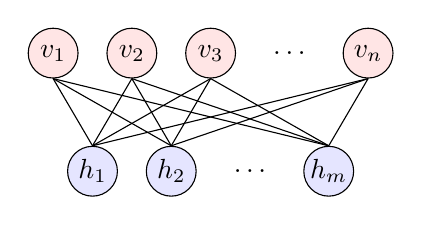
\begin{tikzpicture}
		\node [draw=black, fill= red!10, circle, inner sep=0pt, minimum size=18pt] (v1) at (0,0) {$v_1$};
		\node [draw=black, fill= red!10, circle, inner sep=0pt, minimum size=18pt] (v2) at (1,0) {$v_2$};
		\node [draw=black, fill= red!10, circle, inner sep=0pt, minimum size=18pt] (v3) at (2,0) {$v_3$};
		\node [draw=none] (dots1) at (3,0) {$\dots$};
		\node [draw=black, fill= red!10, circle, inner sep=0pt, minimum size=18pt] (vn) at (4,0) {$v_n$};
		
		
		\node [draw=black, fill=blue!10, circle, inner sep=0pt, minimum size=18pt] (h1) at (0.5,-1.5) {$h_1$};
		\node [draw=black, fill=blue!10, circle, inner sep=0pt, minimum size=18pt] (h2) at (1.5,-1.5) {$h_2$};
		\node [draw=none] (dots2) at (2.5,-1.5) {$\dots$};
		\node [draw=black, fill=blue!10, circle, inner sep=0pt, minimum size=18pt] (hm) at (3.5,-1.5) {$h_m$};
		
		\foreach \v in {v1, v2, v3, vn}
			\foreach \h in {h1, h2, hm}
				\draw (\v.south) -- (\h.north);
	\end{tikzpicture}
	\caption{Graphical representation of an RBM.}
\end{figure}

Furthermore an RBM is assumed to have the Gibbs distribution given by
\begin{align}\label{RBM_gibbs}
P(\textbf{v},\textbf{h})=\frac{1}{Z}\exp(-E(\textbf{v},\textbf{h})),
\end{align}
where the energy $E(\textbf{v},\textbf{h})$ has the form,
\begin{align*}
 E(\mathbf{v},\mathbf{h}) 
 &=- \sum_{i=1}^n\sum_{j=1}^m v_iw_{ij}h_j -\sum_{i=1}^nb_iv_i-\sum_{j=1}^m c_jh_j\\
 &\equiv -\mathbf{v}^T\textbf{W}\mathbf{h} - \mathbf{b}^T\mathbf{v} - \mathbf{c}^T\mathbf{h},
\end{align*}
for some $\textbf{W}\in \R^{n\times m}$, $\textbf{b}\in \R^n$, and $\textbf{c}\in\R^m$.  We have $w_{i,j}$ encodes the interaction potential between $v_i$, and $h_j$ and the $b_i$, $c_j$ encodes the local potential for $v_i$ and $h_j$ respectively. 



\subsection{RBM Likelihood}
Suppose we have data $\mathcal{D}=\{\textbf{v}^1,\dots,\textbf{v}^\ell\}$, we want to find $\textbf{W},\textbf{b}, \textbf{c}$, that maximize the log-likelihood function given by 
\[\mathcal{L}(\theta|\mathcal{D})=\log P(\mathcal{D}|\theta)\]
%\begin{align*}\label{LL_decomp}
%\mathcal{L}(\theta|\mathcal{D})
%=\log P(\mathcal{D}|\theta)
%=\sum_{k=1}^\ell \log P(\textbf{v}^k|\theta)
%=\sum_{k=1}^\ell \mathcal{L}(\theta|\textbf{v}^k).\numberthis
%\end{align*}
As shown in \S 4.2 in\cite{fischer2014training}), the gradient of $\mathcal{L}$ can be written as,
\begin{equation}\label{LL_grad}
\frac{\partial \mathcal{L}}{\partial\theta}=\E_{P_{data}}\left(\frac{\partial E}{\partial \theta}\right)-\E_P\left(\frac{\partial E}{\partial \theta}\right)
\end{equation}
where $P_{data}$ is the empirical distribution of the data. So by taking the patial derivatives with respect to $w_{ij}, b_i,c_j$, we get the gradient updates given by,

\begin{align*}
\frac{\partial \mathcal{L}}{\partial w_{ij}}&=\E_{P_{data}}\left(v_ih_j\right)-\E_P\left(v_ih_j\right)\\
\frac{\partial \mathcal{L}}{\partial b_i}&=\E_{P_{data}}\left(v_i\right)-\E_P\left(v_i\right)\\
\frac{\partial \mathcal{L}}{\partial c_j}&=\E_{P_{data}}\left(h_j\right)-\E_P\left(h_j\right)
\end{align*}

Hinton \cite{hinton2002training} showed that this update also emerges by minimizing the KL divergence between the data distribution and the equilibrium distribution over the visible variables.

Therefore in order to optimize for our model parameters, we need to compute the above expectations, which in general are intractable. We thus resort to approximating them using MCMC. The natural MCMC method for us to use is Gibbs sampling as the bipartite structure of our graphical model tells us that  $v_i \indep v_k \mid \mathbf{h}$ and $h_j \indep h_l \mid \mathbf{v}$. Thus we get the following conditional distributions
\begin{align}\label{RBM_gibbs_update}
	P(v_i = 1 \mid \mathbf{h}) &= \sigma\Big( b_i + \textstyle{\sum_j} w_{ij}h_j \Big), \\
	P(h_j = 1 \mid \mathbf{v}) &= \sigma\Big( c_j + \textstyle{\sum_i} w_{ij}v_i \Big),
\end{align}
where $\sigma(x)=(1+e^{-x}))^{-1}$ is the sigmoid function.

